\chapter{Problemanalyse}\label{ch:ch2label}
I dette kapitel analyseres forskellige problemstillinger, idrætsforeninger står overfor. I forbindelse med dette, analyseres hvilke personer i foreningerne, der er relevante at interviewe i forbindelse med disse problemer. Den efterfølgende undersøgelse leder til en indskrænkning af et problem, som derefter bliver analyseret, med det formål at ende med en problemformulering. \\
Flere gruppemedlemmer i dette projekt har tidligere dyrket sport i en idrætsforening, hvilket har resulteret i en øget baggrundsviden. Grundet denne baggrundsviden er analysen rettet mod traditionelle idrætsforeninger, fremfor foreninger der tilbyder e-sport. Antallet af foreninger der tilbyder e-sport er også mindre end antallet af foreninger, der tilbyder mere traditionelle sportsgrene \citep{e-sport}. Derfor antages der at være rigere mulighed for at finde en traditionel forening med et problem.
\\\\
For at finde et problem i en idrætsforening, er det fordelagtigt at vide hvem der bliver påvirket af et eventuelt problem. Dette bliver i det følgende afsnit undersøgt i en interessentanalyse. 

\section{Interessentanalyse}
Interessenterne er en stor del af projektet, da der skal laves et program specifikt for at løse deres problem. Denne undersøgelse vil blive brugt til at finde en retning for projektet og et mere afgrænset problem, som kan løses. Det er hermed relevant at forstå hvem interessenterne er og hvad deres behov i forhold til problemet og dets løsning er. Derudover er det også vigtigt at forstå hvilke krav de forskellige interessenter har til løsningen.

\subsection*{Bestyrelse}
En af de større interessenter er bestyrelsen. Medlemmerne inden for bestyrelsen er som regel frivillige. Som bestyrelse har de stor indflydelse på projektet, da det er dem løsningen skal hjælpe, og de kommer til at blive direkte påvirket af projektet. Bestyrelsen har brug for en bedre og hurtigere måde at planlægge og organisere fx turneringerne, frivillige eller udstyr på. Ulempen ved dette kan være at, hvis ikke alle bruger systemet, kan der være sammenstød eller uoverensstemmelser med planlægningen. Det vil hermed være svært at holde styr på systemerne, hvis folk ikke bruger det samme program eller planlægningsmetode.\\ 
Gennem samtale med bestyrelsen kan eventuelle problemstillinger belyses. Der kan således uddrages konkrete problemer, som kan løses med et program. Bestyrelsen kan komme med forslag til potentielle egenskaber, der kunne være brugbare for dem. Dette vil ske gennem et semistruktureret interview, hvor interessenten får lov til at dele sine holdninger frit.

\subsection*{Frivillige}
De andre frivillige er også en vigtig interessent, fordi den anvendte planlægningsmetode i klubben har en væsentlig indflydelse på deres arbejdsopgaver. Da det er de frivillige der ofte sidder med planlægningen, er det i deres interesse at den anvendte metode optimeres. På den måde vil et program kunne formindske den tid, der bliver brugt på planlægningen. Deres behov kan hermed påvirke programmets udformning. Ulempen ved at introducere en ny metode, er at de frivillige skal lære at bruge programmet. Fordelen ved programmet vil være at det bliver nemmere og mindre tidskrævende for den enkelte frivillige at planlægge fx turneringer, tidsplaner eller udskiftningen af slidt udstyr.\\
Det er hermed fordelagtigt at kontakte denne interessent, for at få afklaret, hvilke behov der er i forhold til programmet. Dette vil igen gøres gennem et semistruktureret interview.

\subsection*{Medlemmer}
Medlemmerne har en mindre rolle i forhold til, hvordan løsningen udvikles. De har ikke nogen indflydelse på programmet, da det ikke vil være dem der bruger det. De kan dog blive påvirket af programmet, da optimering af klubbens ressourcer kan have en indflydelse på de aktiviteter de deltager i. Hvis programmet ikke bliver brugt ordentligt eller ikke er effektivt nok, vil det kunne få negative konsekvenser for medlemmerne, da der også er tale om potentiel spild af deres tid. Medlemmernes holdninger og ønsker i forhold til løsningen af problemet vil ikke blive taget i betragtning, da det er de frivillige og bestyrelsen, som kommer til at bruge programmet, og ikke medlemmerne.

\subsection*{Forældre}
Forældre til børn der er medlemmer af foreningen, er interessenter med en minimal indflydelse på programmets udvikling. De kommer ikke til at bruge programmet, de vil dog kunne mærke programmets virkning, især hvis der tidligere er sket fejl i planlægningen, og det så går ud over forældrenes tid og lyst til at deltage i aktiviteter. Eksempelvis kan der være problemer med organiseringen af faciliteterne, hvilket kan føre til dobbeltbookning af hallerne. Hvis forældrene i en sådan situation har kørt børnene til aktiviteten, er det spild af både forældrenes og deres børns tid. Sådanne tilfælde kan undgås, hvis man har et fungerende og effektivt program, der kan holde styr på disse ting.
\\\\\\
På baggrund af interessentanalysen udeledes det, at der er forskellige interessenter, som bliver påvirket af programmet. For at få informationer om hvilke problemer en forening kan have, og som kan løses med et program, bliver der afholdt interviews med bestyrelsen og de frivillige. \\
Det er også valgt at der interviewes forskellige slags foreninger. Dette gøres for at have mulighed for enten at finde et unikt problem, eller et bredere problem som flere forskellige foreninger har. De interviewede foreninger er derfor ikke af samme sportsgren.\\
De valgte foreninger er alle omkring 200 medlemmer. Det er ikke nogle af de største foreninger. Dette antages stadig for at være repræsentativt for normale foreninger, da den gennemsnitlige størrelse netop er ca. 200 medlemmer \cite{idraetTal2017}.

\section{Interviews}
Gennem interviewene har tre emner vist sig at være potentielt interessante. Nedenfor gennemgås resultaterne af interviewene, inddelt i disse emner. For referencer til interviewene, henvises der til bilag B-E, som er transskriptioner af hele eller udvalgte dele af hvert interview.

\subsection*{Udstyr}
Under interviewet med Jonas Nielsen fra Aalborg Flyers, fortalte han at der ikke var én specifik person, der var ansvarlig for deres udstyr. I stedet har frivillige et fælles ansvar for at holde øje med udstyret, i forbindelse med hvornår det er slidt og skal udskiftes. Der er ikke noget system for hvordan dette gøres, men Nielsen viste ikke store bekymringer for, at det var et problem.
\\\\
I Farstrup Boldklub deles foreningen og den lokale skole om udstyret, mens klubben har ansvaret for at købe nyt ind. De har en ansvarlig for trøjerne til håndbold, da der ofte kommer harpiks på dem så de bliver ødelagt og skal skiftes ud. 
\\\\
AKG har deres eget udstyr som de deler med folkeskolen. De har dog noget særligt udstyr som de gerne vil holde under opsyn. Ligesom hos Aalborg Flyers, er der heller ikke her én bestemt person, som holder styr på udstyret. Alle kan kontakte bestyrelsen, hvis der er noget der mangler, skal repareres eller udskiftes. 
\\\\
Det meste af Aalborg karateskoles udstyr er noget medlemmerne selv ejer. De få redskaber som foreningen selv har er bl.a. måtter, sparkepuder og ekstra beskyttelsesudstyr. Da omfanget af udstyret er småt og vedligeholdelsen er minimal, mener foreningens formand, Mogens Juul Møller, ikke, at det har været nødvendigt at have et system til at holde styr på disse.
\\\\\\
Generelt for de interviewede foreninger gælder det, at der ikke er et særligt system bag organiseringen af udstyr. Dette kunne potentielt optimeres med et program. 

\subsection*{Frivillige}
Aalborg Flyers har omkring 20 frivillige, hvor nogle få af dem påtager sig et større ansvar. Der er nogle frivillige som fungerer som trænere, mens fx forældre nogle gange hjælper til ved arrangementer. Under turneringer skal der laves en dommerplan over hvilke frivillige, der fungerer som dommer til hver kamp. Dette gøres manuelt, hvor der forsøges at gøre det så praktisk som muligt. Der opleves også problemer med manglen på medlemmer der aktivt melder sig til at hjælpe til. Dette løser de ved at lave planer uden at tage højde for hvornår medlemmerne har tid. Der er på den måde mulighed for internt at bytte tider.
\\\\
I forbindelse med organisering af frivillige i Farstrup Boldklub, nævner Lars Segerstrøm at opgaver bliver uddelegeret gennem mundtlige aftaler. Når der fx i slutningen af en sæson skal vælges trænere, sker det ved at de nuværende trænere får muligheden for enten at fortsætte, eller tage en pause. Hvis der derefter er nogle poster der mangler at blive dækket, går bestyrelsen i gang med at spørge om der er nogle andre fra lokalsamfundet, der har lyst.
\\\\
Ina Breum fra AKG gymnastikforening fortæller at kommunikationen mellem bestyrelsesmedlemmerne og de frivillige ofte sker gennem e-mail eller Facebook. Dog blev Facebook mest brugt til hurtige spørgsmål, da det ikke er alle der har en bruger. På den måde undgår de at der er nogen, som ikke får de vigtige informationer at vide. Derudover er der et bestyrelsesmøde hver anden måned, hvor forskellige emner og foreslag bliver bragt på banen.
\\\\ % [11:55]
Aalborg karateskoles frivillige består hovedsageligt af bestyrelsesmedlemmer og instruktører. Måden hvorpå de frivillige bliver organiseret, er gennem instruktørmøder, hvor der aftales hvem der tager hvilke hold og hvornår. Der er senere mulighed for at bytte internt mellem instruktørerne. Derudover kommunikeres der gennem e-mails. De har hermed ingen systemer til at holde styr på organiseringen af deres frivillige, da det ikke menes at være nødvendigt.
\\\\\\
Foreningerne har hver deres metoder til at organisere deres frivillige på. Disse metoder vil kunne samles til én, hvor man udvikler ét program der har styr på hvem der har ansvar for et bestemt område. På den måde vil man kunne undgå misforståelser og det vil ikke være et problem at der er nogen der ikke havde fx en Facebook bruger. 

\subsection*{Turneringer}
Jonas Nielsen fra Aalborg Flyers gav udtryk for udfordringer med planlægningen af turneringer. Den metode der bliver benyttet nu, er ved at bruge Excel som værktøj. Nielsen fortæller at problemerne opstår, når der skal laves ændringer i den færdige plan. Fx hvis et hold melder afbud, kan det være nødvendigt at lave det hele om, da planen ikke længere vil give mening. Dette resulterer i meget spildt arbejde og tid. Nielsen fortalte også, at han havde oplevet planlægningen til at være fejlet helt: QUOTE. Dette kunne have været undgået, hvis planlæggerne havde et program til at gøre det for dem.
\\\\
Farstrup Boldklub holder også turneringer, hvor de forskellige udvalg står for planlægningen. Der bliver eksempelvis arrangeret stævnedage, hvor der er flere hold, som spiller i løbet af dagen. Ligesom i Aalborg Flyers, bruger Farstrup Boldklub også Excel som værktøj. Det er dog ikke et fast værktøj, da der også planlægges ved nedskrivning i hånden.
\\\\
AKG gymnastik deltager ikke i turneringer. De laver dog opvisninger, hvor det kun er foreningens egne medlemmer der deltager. For disse opvisninger bliver der ikke brugt noget decideret planlægningsværktøj, da de kun skal organisere deres eget hold.  % [14:05]
\\\\
Aalborg karateskole deltager både i store og små turneringer. De store turneringer bliver planlagt et stykke tid før, hvor de mindre turneringer fastsættes dagen forinden. Planlægningen af turneringsplanerne sker igen i Excel. 
\\\\\\
Den måde hvorpå der planlægges, sker generelt manuelt, hvor der enten bruges Excel eller også foregår det i hånden på papir. Dette kunne optimeres gennem et system, der også vil gøre det nemmere at foretage ændringer i kampprogrammer, uden større vanskeligheder.
\\\\\\
På baggrund af interviewene er der blevet fundet problemstillinger i emnerne udstyr, frivillige og turneringer. Det er blevet valgt at afgrænse fra problemerne om udstyr, fordi problemer med slidt udstyr er trivielt nok til at kunne blive holdt under opsyn med papir og blyant, og kræver ikke mange kræfter at skrive ned. \\
På samme måde afgrænses der fra organisering af frivillige, da det ene af problemerne i forbindelse med frivillige stammer fra mangel på en hjælpende hånd fra de andre frivillige, og det er derfor minimalt hvad hjælp man kan komme med gennem et program.Det andet problem kommer i forbindelse med at de forskellige foreninger alle bruger forskellige metoder til organisering af de frivillige, dog virker dette ikke til at være et stort problem, da foreninger sagtens kan organisere sig gennem deres nuværende metoder. \\
Der er derfor blevet afgrænset til turneringer. Dette er gjort fordi turneringsplanlægning er et konkret problem, som kunne blive forbedret ved hjælp af et program. Samtidig er turneringsplanlægningen et specifik og afgrænset område, som ikke er et trivielt problem, hvis der hele tiden skal ændres i planen.


\section{Turneringer}
Der findes rigtige mange forskellige former for turneringer. De har næsten alle det samme formål at finde den bedste i sportsgrenen, men de bliver udført på forskellige måder. Et eksempel kunne være i karate, hvor man kan dyste om hvem der er bedst til at lave øvelser af varierende sværhedsgrad[Kilde, bilag]. Samtidig spiller man i fodbold mod hinanden, for også at finde den bedste, men det er mere direkte end karate. Det er generelt set den samme turneringstype, men der er små forskelle på alle sportsgrene, med forskellige traditioner og regler for op- og nedrykning. Derfor vil der i denne rapport blive fokuseret på floorballs regler for turneringer, og deres traditioner. 
\\\\
Undtagelsen til turneringerne med det formål at finde den bedste, er turneringerne for børn. Disse handler mest om at børnene skal have det sjovt, og lære sporten at kende, så de får typisk ikke point, og der er derfor ingen reel vinder [Kilde, bilag]. 


\subsubsection{Landsturneringer}
Landsturnering i Floorball er en landsdækkende turnering der løber gennem en hel sæson. Den begynder i september og slutter i april[Kilde]. Turneringen er delt op i to regioner – vest og øst. Denne opdeling kan variere, alt efter hvor mange hold der er, og hvilken sportsgren der er tale om. 
\\\\
I hver sportsgren er der mange divisioner der er på forskellige niveauer, hvilket også er gældende i floorball [Kilde?]. Kun de øverste divisioner har opryknings- og nedrykningskampe, hvilket er med til at bevare det høje niveau. Eksempelvis kan de hold i den næstbedste division som suverænt er bedst, have mulighed for at gå videre til den bedste division ved at spille disse oprykningskampe. Det samme er gældende for de hold i den bedste division der ligger nederst på pointtavlen og taber alle kampene. Hold kan rykkes op og ned i divisioner, og det gør, at der ikke er for stor forskel på niveauet mellem holdene.
\\
% Billede
\begin{figure}[H]
  \centering
  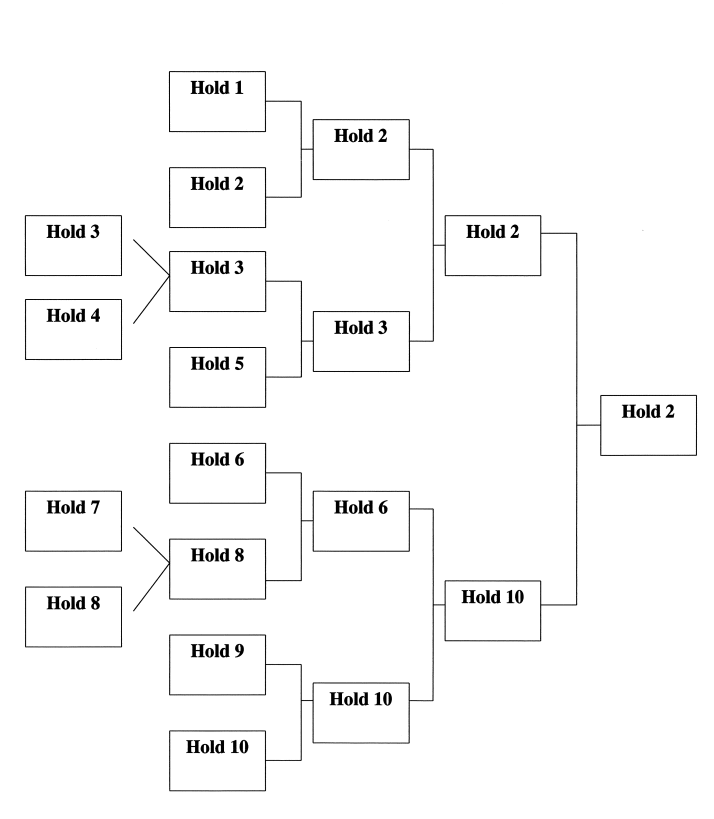
\includegraphics[width=0.7\textwidth]{figures/cup-spil.png}
  \caption{NOGET ANDET BESKRIVELSE 
  \citep{REFERENCE}.}
  \label{fig:test}
\end{figure}

Kampe afvikles ved brug af et cup-system (billede, kilde). Der er først et grundspil, hvor alle hold bliver opdelt i et antal af puljer, og så bliver der spillet indbyrdes. Derefter skal de bedst placerede i hver pulje dyste mod hinanden, hvilket vil afgøre hvilke fire hold der skal gå videre til at spille imod de fire bedste hold fra den anden region. Vinderne går videre til næste runde, og sådan forløber resten af turneringen indtil der er to finalister tilbage.
Sidst på sæsonen vil der være en finale, for at afgøre vinderen af de to resterende hold. Landsturneringer varer en hel sæson, så der er meget der skal laves både før- og imens sæsonen er igang. Nielsen fra Aalborg Flyers siger, at deres bestyrelse bruger meget tid på at få det hele til at fungere [kilde]. Det er ikke kun forbundet der arbejder med turneringen - idrætsforeningerne er meget involveret i planlægningen gennem hele sæsonen. (citat: linje 148 i bilag C) 

\subsubsection*{Pokalturneringer}
I modsætning til landsturneringerne, er alle regler om divisioner og deres niveau ophævet i pokalturneringen. Dette  gør turneringen tilgængelig for alle hold, uanset hvilken division de er i. Pokalturneringen gør også brug af cup-systemet, men turneringen afvikles hurtigere. Pokalturneringen varer ikke hele sæsonen. Den begynder i august og er færdigafviklet i januar måned. Nielsen havde ikke en mening om pokalturneringen, fordi det ikke var hans område, men det antages at denne turnering også tager tid til at planlægge. Den har meget tilfælles med landsturneringer, men den er kortere, så den tager tid at planlægge, men ikke lige så meget som landsturneringen gør.
 
\subsubsection{Stævner}
% Vi skal være enige om vi vil bruge "stævner" eller "1-dagsturnering"
De ovenstående turneringstyper er ikke gældende for børn i Floorball. I de seneste år har der været mere fokus på at få flere børn til at spille, samtidigt med at få flere børn til at dyrke idræt (kilde). Det har forbundet formået at gøre, ved at introducere stævner. Stævnerne er mere hyppige end de andre turneringer, og bliver  afviklet i løbet af én dag, som foregår i weekenderne. Der er flere måder at afvikle stævnerne på. Ældre årgange bruger cup-systemet, og for børn bliver stævnet afviklet ved hjælp at et nyt koncept, som de seneste par år har floreret(et andet ord) i Danmark. Det er et koncept, der bruges af flere sportsgrene, som er tilrettet til børn.
Floorball har, som en af flere sportsgrene, lavet en KidzLiga, som følger det fokus. I ligaen er der niveauinddeling, hvor børnene bliver sat på niveauer, som matcher deres sportskompetance. Dette er en ny måde at opdele spillere på ift. til den traditionelle måde, hvor der blev opdelt efter alder. 
Børnene spiller i mindre baner, og hver kamp bliver afviklet på 6 minutter. Der kan ikke optjenes point til stævnerne, hvilket gør at der ikke er nogen vindere eller tabere i ligaen. 
\\
Selvom om ældre også kan deltage i stævner, er det oftest ungdommen som deltager regelmæssigt hos Aalborg Flyers, som Nielsen også siger: 
\\\\
\say{Ja, altså for ungdom er det sådan meget de her én-dags som er cirka én gang om måneden.} (Bilag C)
\\\\
Som der blev sagt ovenfor, foregår stævnerne hver måned, og idrætsforeningerne skiftes om at være vært (Bilag C). De bestemmer selv hvordan deres eget stævne skal organiseres, men hvis de ikke vil bruge tid på planlægning af kampene på stævnedagen, kan forbundet tage sig af det. Dette sker ikke ofte, og ifølge Nielsen planlægger Aalborg Flyers deres stævner selv (bilag c). Før sæsonen begynder, planlægger idrætsforeningerne sammen med forbundet, hvornår alle hver især skal holde stævne, hvilket giver bestyrelserne god tid til at planlægge og organisere faciliteter til stævneerne (omformuleres). 
\\\\ % Hvorfor har vi valgt 1-dagsturneringer?\\
De store lands- og pokalturneringer planlægges af forbundet. Da denne planlægning er ude af foreningernes hænder, fravælges det her at fokusere på dem. I stedet, vil der blive fokuseret på 1-dagsturneringer, da disse bliver planlagt og organiseret af den lokale forening. Der er også mulighed for at foreningen kan overlade planlægningen til forbundet, men ud fra de interviews der er blevet foretaget, er der fundet eksempler på at planlægningen bliver udført lokalt. Denne planlægning er ikke altid lige god, og det vil derfor være et godt sted at fokusere på [kilde].
  
\subsection*{Planlægning af 1-dagsturneringer}
I dette afsnit beskrives det hvordan en 1-dagsturnering eller stævne i KidzLiga floorball arrangeres. Denne måde at planlægge og afvikle en tunering på, kan gælde for andre sportsgrene, men dette afsnit omhandler kun KidzLiga floorball.
\\
\\
Floorball Danmark er et specialforbund, med det formål at give interesserede personer mulighed for at spille floorball. En forening der ønsker at arrangere et KidzLiga-stævne, kan vælge at indsende en formular til Floorball Danmark, hvorefter de arrangerer det, eller foreningen kan arrangere stævnet på egen hånd. Stævnerne arrangeres lokalt eller regionalt, og forbundet forsøger at afholde mindst ét stævne i måneden, i hver region. Ved sæsonens afslutning afholdes der et stævne, hvor det er muligt for deltagere fra alle regioner at deltage.\\
Floorball Danmark tager sig af promovering og tilmelding til stævnet. Derudover udarbejder de et kampprogram der tilsendes værtsforeningen fem dage før stævnet. Foreningen har herefter mulighed for selv at redigere programmet, og har pligt til at rette det til, i tilfælde af afbud.\\
Foreningen skal selv sørge for, at der er udstyr tilgængeligt, og at der bliver opstillet baner. Det er også værtsforeningen der skal afvikle stævnet, ved eksempelvis at have dommere til kampene, og sørge for at der er tilstrækkeligt mandskab\citep{kidzRegler}. 
\\\\
Aalborg Flyers arrangerer selv deres 1-dagsturneringer. De sender selv invitationer ud til andre floorball foreninger, ofte via Facebook eller mail. De arrangerer også turneringer for skoler, bl.a. til Skolernes Floorball Dag. Ved planlægning af disse, inddeler Aalborg Flyers de tilmeldte hold efter alder, og evt. i puljer indenfor hver aldersrække hvis nødvendigt. Til opstilling af programmet bruges en skabelon i Excel. Dette kan være et stort arbejde, især hvis der senere skal laves ændringer i programmet.
\\\\
Ligegyldigt om programmet for en turnering er planlagt af Floorball Danmark eller den enkelte floorball forening kan det være tidskrævende og besværligt at skulle redigere det i tilfælde af afbud, især når de først får besked på dagen af turneringen. 


% Hvad skal man tage højde for?\\
 % - Regler\\
 % Der er et link på Discord om reglerne i Kids floorball\\
   % - Yngre og ældre spillere\\
   % - Kids koncept\\
     % - Kampe tager 6 minutter "løbende tid"
     % - 1-2 minutters pause mellem kampe
     % - Skal have en hvilekamp mellem hver kamp, hvis ikke muligt skal kampene gerne    foregå på samme bane.
     % - Alle kampe skal starte og slutte på samme tid
     % - Der er forskellige niveauer, indeles efter skills og ikke alder.
 % - Afmeldinger\\
 % Der opstår problemer i planlægningen, når folk melder fra\\
 % - Andre ting\\
 % floorball.dk/staevner/
 
 
\subsection{Eksisterende planlægningsmetoder}
Excel (Tager ikke højde for flere kampe i træk)\\
Challonge (https://challonge.com/)\\
Cup Fixture Generator (https://www.daftlogic.com/projects-cup-fixture-generator.htm)\\ 
Tournament scheduler (http://tournamentscheduler.net/) (Round Robin Only!)\\
Teampolis - Round Robin (https://www.teamopolis.com/tools/round-robin-generator.aspx)\\

Online generatorer:
Hvad har disse værktøjer tilfælles? Hvad kan de ikke?

Der opstår problemer i planlægningen, når folk melder fra.
